%Die Angabe des schlauen Spruchs auf diesem Wege funtioniert nur,
%wenn keine Änderung des Kapitels mittels den in preambel/chapterheads.tex
%vorgeschlagenen Möglichkeiten durchgeführt wurde.
\chapter{Faults in VLSI Systems}
\label{chap:chapter2}
%\vspace{-3cm}
%\vspace{2cm}

The reliability is always a cause of concern during chip manufacturing. A manufactured chip needs to function correctly not just during post-manufacturing tests but during the complete lifespan of the final product. The typical lifespan for a chip designed for commercial purpose is defined as 11.4 years or 100,000 hours \cite{kishore2009}. The failure rate of ICs with respect to time is shown in figure~\ref{fig:bathtubcurve}, typically known as the \emph{bathtub curve}.

\begin{figure}[h]
  \begin{center}
    \captionsetup{justification=centering}
    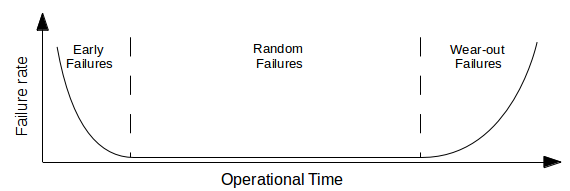
\includegraphics[scale=0.5]{figures/bathtubcurve.png}
    \caption{Bathtub Curve}
    \label{fig:bathtubcurve}
  \end{center}
\end{figure}

The first region of the graph is called early failures or \emph{infant mortality region}. The second region is the lifetime of the device when random failures occur. The error rate in this region is low and constant. The third region of the graph is wear-out and is caused by failures at the end of the useful life \cite{kishore2009}. It can be expected that the ICs will not enter this region due to technology advances and obsolescence. This makes the first region important from the view of product quality. Early failures of chips can be remedied to a great extent by testing them immediately after manufacturing \cite{Agrawal2000} and thus it is important to detect faults at the manufacturing level.

Failure of a semiconductor chip can be described using a fault, defect or an error. A \emph{defect} in an electronic system is an unintended difference between implemented hardware and its design \cite{Agrawal2000}. Defects can occur either during the manufacturing process or lifetime of the device. An \emph{error} is said to have occurred when an unintended signal is generated by the system. An error may result in failure at primary outputs of the system. An error is essentially the manifestation of a defect. For the purpose of analysis, a defect is modeled as a \emph{fault}, which is simply representation of defect at the abstracted function level.

\begin{figure}[h]
  \begin{center}
    \captionsetup{justification=centering}
    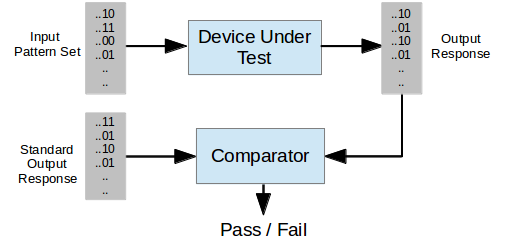
\includegraphics[scale=0.75]{figures/vlsitesting.png}
    \caption{Typical test flow for VLSI Chips}
    \label{fig:vlsitesting}
  \end{center}
\end{figure}

The figure~\ref{fig:vlsitesting} shows how faulty chips are identified. To decide whether the Device Under Test (DUT) is working properly, a set of input stimuli called \emph{test pattern set} is applied to the DUT. The \emph{output response} is observed and is then compared to the standard output. If these outputs do not match then the chip is said to be faulty.

The sources of the fault can be either internal or external. When healthy chips fail due external mechanisms like $\alpha$-particle strikes, they are thrown away in a typical test, which contributes to yield loss. Thus to maintain product quality and to reduce yield loss, it is important classify the faults according their criticality. Section 2 of this chapter describes a taxonomy for such classification according to their sources and characteristics. It also focuses on various fault models that can be used to analyze these faults. The existing techniques for such fault classification are explained in section 3. The last section of this chapter explains diagnostic techniques and how they can used to classify faults.

\section{Fault Taxonomy}
\label{sec:secft}
According to the source and behavior of faults, they can be classified into three types: \emph{permanent}, \emph{intermittent}, and \emph{transient} \cite{Constantinescu2003}. Permanent faults reflect irreversible physical changes. Intermittent faults occur because of an unstable or a marginal hardware, and can be activated by environmental changes, like higher or lower temperatures and voltage. Transients occur because of temporary environmental conditions \cite{Constantinescu2003}. The likelihood of these faults is expected to increase with increase in transistor densities on semiconductor chips \cite{Constantinescu2007}.

\subsection{Permanent Faults}
Permanent faults are those which occur due to physical defects on the chip. The source of these faults generally lies in the issues of manufacturing process. However, they can also occur during operational lifetime of the circuit, especially when circuit is old and starts to wear-out.

The common sources of permanent faults are described below:
\begin{description}
\item[Manufacturing process:] Sso-called \emph{spot defects} can occur during manufacturing of a VLSI chip, and take form of either missing or extra material. Such a defect can cause an unwanted short or open between nodes or make an unintended multi-terminal transistor,leading to changed circuit topology. These defects mainly arise from some contamination, usually in form of dust particles or liquid droplets deposited on the wafer surface during some fabrication step \cite{Khare1996}. Also missing or excess metal may cause unwanted capacitance and resistance respectively resulting in delay lines \cite{Wagner1995}.

\item[Wear-out:] \emph{Electromigration} (EM) is defined as mass transport of metal atoms created by collision of electrons \cite{Ghate1982}. This movement of material will result in voids or hillock growth as in figure~\ref{fig:mfgdefects}, which can result in an open circuit or a short between adjacent tracks \cite{AnalogDevices2000}. With lower technology nodes, the wire widths are also getting smaller making EM a serious problem.
\end{description}

\begin{figure}[h]
  \begin{center}
    \captionsetup{justification=centering}
    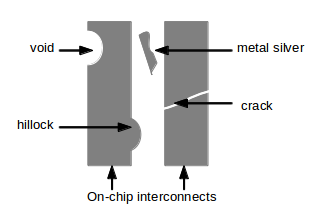
\includegraphics[scale=0.75]{figures/mfgdefects.png}
    \caption{Manufacturing defects as sources for intermittent and permanent faults \cite{Lehtonen2009}.}
    \label{fig:mfgdefects}
  \end{center}
\end{figure}

Once a permanent fault appears in the system, it does not go away, unless the offending component is replaced. They are localized on the chip, and hence will affect the same set of primary outputs (POs). Permanent faults are reproducible and provide a predictable output response. Permanent faults only go away once the offending component is replaced \cite{Constantinescu2007}.

Some of the ways to model permanent faults are noted below, these are the models used to generate experimental data in this work.
\begin{description}
\item[Stuck-at fault model:]
Stuck-at fault models are the most simplest fault models. Due to its simplicity it is a widely used fault model\cite{Larsson2006}. It assumes that the fault location has a fixed logical value, either stuck-at 0 or stuck-at 1. These can be seen as short to ground or short to power supply respectively. When it is assumed that there is only one fault in the circuit at a time then \emph{single stuck-at} (SSA) model is used, otherwise in case of multiple defects \emph{multiple stuck-at} model is used.

\item[Wired AND/OR fault model:]
Unlike stuck-at, \emph{bridge fault} models a short between signal lines. \emph{Wired AND/OR} fault model is a type of the bridging fault model. These models are used to describe the logic behavior of two nodes that are shorted in the circuit. Wired AND model assumes that the faulty node of the bridge always has value 0, whereas wired OR model assumes faulty node has value 1. 

\item[Delay fault model:]
\emph{Delay fault} model is used to model timing related faults. Delay testing is required for modern VLSI systems running at high frequencies, as even minor timing violations can lead to system performing out of specifications \cite{Larsson2006}. There are two was to realize delay viz. \emph{Gate delay} and \emph{Path delay} models. Gate delay model assumes that the delay is only between input and output of individual logical gates on chip. In contrast, path delay models assume that the delay is spread over complete path from input to output. 
\end{description}
\subsection{Intermittent faults}
\label{sec:secif}
Intermittent faults are those caused by a marginal or an unstable hardware and are activated when certain conditions like voltage, temperature or frequency are met \cite{Constantinescu2003, Lehtonen2009}. Intermittent faults often precede occurrence of permanent failures \cite{Lehtonen2009}.

Some of the common sources for intermittent faults are described below:
\begin{description}
\item[Manufacturing defects:] As illustrated in figure~\ref{fig:mfgdefects} \emph{metal silvers} are stray pieces of metal on die due to some process imperfections. In certain conditions like increase in temperature, the metal may expand and touch the interconnects creating a short. In some cases the short might cause a current surge, damaging the circuit and can manifest into a permanent fault \cite{Hawkins2003}. Similarly cracks, as shown in same figure can continue to work normally at design temperature but at low temperatures can cause open circuits.

\item[Technology scaling:] With the technology scaling, the reduced thickness of oxide layers may result in current leakage, with a mechanism known as soft breakdown (SBD) \cite{Stathis2001}. In such a breakdown, the current fluctuates creating intermittent fault, without causing a thermal damage \cite{Stathis2001, Constantinescu2007a, Constantinescu2007}. 

\item[Power droop:] With the technology scaling, supply voltages are also lowered down, this results in degraded tolerance to power supply noise resulting in a \emph{low frequency power droop}\cite{Polian2007}. A \emph{high frequency power droop} occurs when multiple cells on a chip connected to the same power grid segment switch in the same direction, increasing their current demand causing a power starvation in some other part of chip \cite{Polian2007}. 
\end{description}

Once intermittent fault appears in the system, its probability of recurrence increases with time\cite{Bondavalli2000}. These faults are localized on the chip. They will affect the same set of primary outputs (POs) on recurrence. Intermittent faults have tendency to occur in bursts \cite{Constantinescu2007, Constantinescu2003}. Intermittent faults are not reproducible every time for same set of test patterns. Intermittent faults only go away once the offending component is replaced \cite{Constantinescu2007}.

Intermittent faults can be modeled as conditional stuck-at faults, activated by trigger condition. The activation condition can be expressed as a Boolean function and can depend on timing or environmental conditions \cite{Holst2009}.

\begin{description}
\item[High frequency power droop:] This type of fault occurs when specific set of input causes power starvation in some other part of the chip. Hence, this fault is modeled as a set of aggressor lines $a_1,a_2,...$ and a victim line $v$ \cite{Polian2007}. The fault occurs on victim line, due to presence of the aggressor lines.
\end{description}

\subsection{Transient faults}
\label{sec:sectf}
Transient faults are  deviations of normal circuit function caused by some  environmental factors or some external phenomenon. They are called soft errors as they do not do any permanent damage to the chip. A \emph{single-event upset} (SEU), which is change in value of single bit, is the most common manifestation of transient faults.


Some of common sources for transient faults are noted below:
\begin{description}
\item [ESD and EMI:] \emph{Electromagnetic interference} caused by sources emitting high energy signal may interfere with the working chip to bring about SEUs. An \emph{electrostatic discharge} due to users releasing static charge can also affect chips to cause transient faults.

\item[Particle strikes:] When an $\alpha$-particle, a proton or a neutron passes through a semiconductor material and starts to loose energy, it frees electron-hole pairs along its path \cite{Dodd2003}. If this material happens to be a reversed biased p-n junction, it can result in significant transient currents to bring about an SEU. Hence with scaling to lower technology nodes, it is very likely that probability of such SEUs will increase.

\end{description}


Transient faults are non-deterministic faults. These faults are not localized hence can affect any of the POs. Transient faults are not reproducible. Replacing the offending component may not make transient faults to go away \cite{Constantinescu2007}. Transient faults are isolated incidences of error occurrence. They usually do not occur in bursts like intermittent faults \cite{Constantinescu2007, Constantinescu2003}. Once the condition triggering the transient fault disappears, circuit return to normal functioning.

One of the ways  to simulate a transient fault is to implement a conditional stuck-at fault, at multiple fault location and to use a deterministic function to trigger the fault. This work uses a bit-flip as a fault model to model transient faults.

\begin{description}
	\item[bit-flip] A bit at random location is flipped using a trigger condition. This corrupted in value is then propagated through circuit \cite{Gracia2001}. 
\end{description}

\section{Fault Classification}
\label{sec:secfc}
Test flows like the one shown in figure~\ref{fig:vlsitesting} are able to distinguish between faulty and healthy chips. The traditional manufacturing tests still work the way as shown in figure~\ref{fig:traditionaltestflow} \cite{Weste1985}. Chips are tested for faulty behavior, and all chips showing single fault in a test run are thrown away.

\begin{figure}[h]
  \begin{center}
    \captionsetup{justification=centering}
    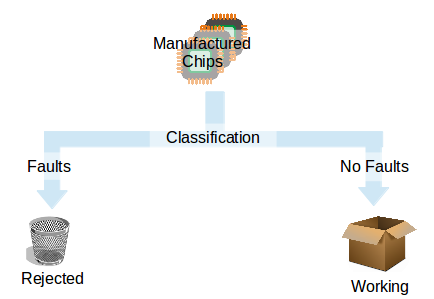
\includegraphics[scale=0.75]{figures/traditionaltestflow.png}
    \caption{Traditional flow for fault classification}
    \label{fig:traditionaltestflow}
  \end{center}
\end{figure}

With the advances in manufacturing processes, the number of permanent faults is increasing \cite{kishore2009}. However, on the other hand the impact of soft-errors and other non critical failures is increasing at much higher rate\cite{Constantinescu2003}. Some studies have indicated that up to 80\% failures can be attributed to SEUs \cite{Iyer1986, Dharchoudhury1994, kishore2009}, which suggest that these cases will result in an unnecessary yield loss. This section describes a few techniques to discriminate between different error categories described earlier in the chapter. As the fault taxonomy we used is similar in characteristics to those observed on PCs or workstations, the approaches used for their classification also provide a few pointers towards fault classification in VLSI systems. 

In \cite{Lin1990} a mechanism to classify between transient and intermittent faults is explained for error log analysis. In a technique called \emph{Dispersion Frame Technique} (DFT), the inter-arrival time in between successive error events of same error types is used to determine type of the fault in the system. Heuristics are applied to determine their closeness in time and affected area, which are then considered as parameters to decide whether the error is of the same type.

Authors in \cite{Iyer1990} use a similar technique to identify persistent failures in the system. Here they have used error rates to build up correlation using simple probabilistic techniques between error records, leading to a set of symptoms which may suggest a common cause (permanent errors).

A probabilistic approach is considered in \cite{Pizza1998}, which updates the probability of module being affected by permanent fault. It then weighs the consequences of actions performed by a faulty module against a fault-free module. It uses Bayesian inference to discriminate between permanent and transient errors

Historically a lot of work has been done to analyze impact of different types of faults on VLSI systems \cite{Constantinescu2003,Constantinescu2007,Dodd2003} and to classify them \cite{Savir1980, Espinosa2013, Bondavalli2000, DeKleer2009}.

The most popular techniques to classify transients from other types of faults are grouped under a family called $\alpha$-count techniques \cite{Bondavalli2000}. In a scheme called \emph{single threshold $\alpha$-count techniques}, a single threshold is established and if error count exceeds this threshold then the fault is classified as permanent or intermittent, whereas a smaller non-zero value indicates presence of transient faults. In an other variant of the same called \emph{dual threshold $\alpha$-count techniques}, two thresholds are established. If the error count exceeds first threshold then that component is assigned a restricted functionality and when it exceeds the second threshold it is taken out of service, like the single threshold technique. However, a component which is in-between thresholds can be taken in full service once its error count is lowered than first threshold.

Another approach using diagnostic probabilities in \cite{DeKleer2009} is able to distinguish permanent faults from faults with non-deterministic behavior.

\section{Fault Diagnosis}
\label{sec:secfd}
\emph{Diagnosis} is the process of locating faults in a physical chip at the various levels down to real defects. In the traditional fault-dictionary based diagnosis, we are given two sets of data, a \emph{predicted output} $P$ which is a set of outputs when fault a particular fault is active in the system, a \emph{measured set} $M$, which is the observed fault behavior and corresponding fault $ f_i \in \{f_1,f_2,...,f_n\} $. When the two sets match i.e. $P = M$ the corresponding fault is diagnosed to be active . When $P \neq M$ then logic diagnosis tries to find the best fitting explanation. However it is practically infeasible to construct such fault dictionaries for modern circuits, as the fault dictionary should consist of all possible faults and their combinations \cite{Wang2010}. 

An adaptive approach which does not use fault dictionaries called \emph{Partially Overlapping Impact couNTER} (POINTER) for diagnosis is described in \cite{Holst2009}. This approach uses test pattern sets with the \emph{Single Location At a Time} (SLAT) property \cite{Bartenstein2001} to diagnose faults present in the circuit. The authors in \cite{Holst2009} define a \emph(Fault Machine) (FM), \emph{i.e.} a reference circuit with stuck-at faults injected. As shown in figure~\ref{fig:evidance}, a tuple of parameters called \emph{evidence} is defined as,

\[e(f,T) = \{\sigma_T, \iota_T, \tau_T, \gamma_T\}\]. 

\begin{description}
	\item[$\sigma_T$] is the sum of number of failing output  where the Device Under Diagnosis (DUD) and the FM match. It is calculated as sum of all $\sigma_t$ values by injecting one stuck-at fault at a time in the FM.
	\item[$\iota_T$] is the sum of number of output pins which fail in the FM but are correct in the DUD. It is calculated as sum of all $\iota_t$ values by injecting one stuck-at fault at a time in the FM.
	\item[$\tau_T$] is the sum of number of output pins which fail in the DUD but are correct in Fthe M. It is calculated as sum of all $\tau_t$ values by injecting one stuck-at fault at a time in the FM.
 	\item[$\gamma_T$] is the sum of maximum of corresponding values of $\iota_t $ and $\tau_t$ for every test pattern.
\end{description}

\begin{figure}[h]
  \begin{center}
    \captionsetup{justification=centering}
    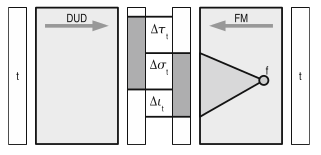
\includegraphics[scale=1.00]{figures/evidance.png}
    \caption{Evidence generated during diagnosis \cite{Holst2009}}
    \label{fig:evidance}
  \end{center}
\end{figure}

The values of $\iota$ and $\tau$ are high and $\sigma$ is low or zero, if the fault present in DUT is not explainable using any of the stuck-at faults injected in FM. Hence $\gamma$ is an indication about the ability to explain of the fault. For a permanent fault, the value of gamma would be low (zero). 

After diagnosis, in a process called \emph{ranking} obtained values are sorted as evidence with lowest value of $\gamma$ first. The evidences with the equal values of $\gamma$ are then sorted with the highest value of $\sigma$ first. For evidences with equal values of both $\sigma$ and $\gamma$, the ranking algorithm puts evidences with lowest value of $\iota$ first \cite{Holst2009}. This process brings the most explainable faults first. The result of diagnosis is then returned as the evidence with the highest rank.

These parameters vary depending on the type of fault present in the circuit. For permanent faults, the value of evidence parameters remains same, when same test pattern is applied at the input. The evidence would vary for each test run, as intermittent and transient faults are non-deterministic.



